\documentclass[a4paper]{article}

%% Language and font encodings
\usepackage[english]{babel}
\usepackage[utf8x]{inputenc}
\usepackage[T1]{fontenc}

%% Sets page size and margins
\usepackage[a4paper,top=3cm,bottom=2cm,left=3cm,right=3cm,marginparwidth=1.75cm]{geometry}

%% Useful packages
\usepackage{amsmath,parskip,palatino, graphicx}
\usepackage[colorinlistoftodos]{todonotes}
\usepackage[colorlinks=true, allcolors=blue]{hyperref}

\setlength\parindent{0em}


\title{M.S. Writing Project}
\author{Andrea Mack}

\begin{document}
\maketitle

%\begin{abstract}
%Your abstract.
%\end{abstract}

\section*{Schedule}

\begin{table}[h!]
\centering
\begin{tabular}{c|c}
Week of & Tasks \\\hline
Jan 23 & \begin{tabular}[t]{@{}c@{}}Review Ch.2 Banerjee, Carlin, \& Gelfand \\
Look at R software for simulating and fitting variograms. \end{tabular}  \\
\hline
Jan 30 & \begin{tabular}[t]{@{}c@{}} Simulate data with known covariance structure \\ Fit Bayesian spatial model to simulated data \\ Start annotated bibliography  \end{tabular}\\
\hline
Feb 6 & \\
Feb 13 & \\
Feb 20 & \\
Feb 27 & \\
Mar 6 & \\
Mar 13 & \\
Mar 20 & \\
Mar 27 & \\
Apr 3 & \\
Apr 10 & \\
Apr 17 & \\
Apr 24 & \\
Apr 31 & Writing Project Due:\\
\hline
\end{tabular}
\caption{\label{tab:schedule}Writing Project Schedule}
\end{table}

{\bf I don't think overleaf supports r code, perhaps use gitlab}



\section*{Package Exploration}
<<code>>=
require(geoR)
http://leg.ufpr.br/geoR/geoRdoc/geoRintro.html


se <- read.csv("SEDataForAnalysisSpSurveyFinal.csv")
head(se)

#The fields you are likely interested in for now are the xcoord, ycoord 
#(locations for the sample points); SiteID the unique id for a survey location; 

#mdcaty.x = refers to the water zones within a management unit: 
#flooded, saturated, intermittent; stratum.x = the unit name on the refuge so the different management units;

#Acres and Hectares are the size of the areal frame within each of those water zones within a unit; 
#Date_ = survey date when the data was collected;
#SeSed is selenium concentration within a sediment sample;
#SeRoot is selenium concentration within a root sample; 
#SeWater is selenium concentration within a water sample; and 
#SeBugs is selenium concentration within a bug sample.



se.cols <- c("siteID", "xcoord", "ycoord", "mdcaty.x", "Date_", "Acres", "Hectares", 
             "SeSed", "SeRoots", "SeWater", "SeBugs")

se_sub <- se[,se.cols]

#rep.data.action = "first" keeps only first coordinate pair if same coordinate
#pair represented more than once in dataframe
se_geo <- as.geodata(obj = se_sub, coords.col = c(2,3), 
                     data.col = c(8:11), covar.col = c(1,4,5,6,7), 
                     na.action = "none")

summary(se_geo)
#diff number of NAs in each group

plot(se_geo, col.data = 1)
#won't work bc of all the NAs

geo_all <- as.geodata(obj = se_sub, coords.col = c(2,3), 
                     data.col = c(8,9,10,11), 
                     covar.col = c(1,4,5,6,7), 
                     na.action = "none")
#I don't know what the colors mean... 
#documentation says they are the four "Quartiles"
#do they mean the four quantiles?
#quantiles of what?
#I am thinking of the coordinates?

## need to figure out how to do this with all data
plot(geo_all, na.rm = TRUE)
#showing higher se concentration 
#where the authors suggested, units 1 and 2 = low x coord and high y coord

sed_geo <- as.geodata(obj = se_sub, coords.col = c(2,3), 
                      data.col = c(8), 
                      covar.col = c(1,4,5,6,7), 
                      na.action = "ifdata")

plot(sed_geo)
points(sed_geo, pt.divide = "rank.prop")
#shows it more clearly

## continuing from
## http://www.leg.ufpr.br/geoR/geoRdoc/vignette/geoRintro/geoRintrose3.html
## eda plots


# variogram with classical estimator
# switch to modulus estimator by estimator.type = "modulus"
sed_cloud <- variog(sed_geo, option = "cloud")
sed_bin <- variog(sed_geo, uvec = "default")

par(mfrow=c(1,2))
plot(sed_cloud, main = "Cloud Variogram")
plot(sed_bin, main = "Binned Variogram")

# create a "binned" cloud variogram
sed_cloudbin <- variog(sed_geo, uvec = "default",
                       bin.cloud = TRUE)
plot(sed_cloudbin, bin.cloud = T, main = 
       "Classical Estimator, Binned Cloud Variogram")

## directional variograms, angles = 0,45,90,135
## tolerance at default of 22.5 degrees

## resource on interpretting variogram and quality measures

par(mfrow=c(1,1))
sed_vario4 <- variog4(sed_geo)
plot(sed_vario4)

## parameter estimation
## theoretical vs. empirical

plot(sed_bin)
lines.variomodel(cov.model = "exp", cov.pars = c(1,2),
                 nugget = 4)

sed_smooth <- variog(sed_geo, option = "smooth")#, ksmooth = "normal")
lines(sed_smooth, type = "l", lty = 2)
legend(0.4,0.3,c("empirical", "exponential model", 
                 "smoothed"), lty = c(1,1,2), lwd = c(1,3,1))


plot(variog(sed_geo, max.dist = 1)) 
lines.variomodel(cov.model = "exp", cov.pars = c(1, 
                                                   0.3), nug = 0, max.dist = 1) 
lines.variomodel(cov.model = "mat", cov.pars = c(0.85, 
                                                     0.2), nug = 0.1, kappa = 1, max.dist = 1, 
                     lty = 2) 
lines.variomodel(cov.model = "sph", cov.pars = c(0.8, 
                                                      0.8), nug = 0.1, max.dist = 1, lwd = 2)
#ml or reml parameter estimation for
#gaussian random fields
sed_ml <- likfit(sed_geo, ini.cov.pars = c(1,1))
summary(sed_ml)

# no nugget
options(geoR.messages = FALSE)
sed_ml <- likfit(sed_geo, ini = c(1,0.5),
                  fix.nugget = T)
sed_reml <- likfit(sed_geo, ini = c(1,0.5),
                   fix.nugget = T,
                   method = "RML")

sed_ols <- variofit(sed_bin, ini = c(1,0.5), 
                    fix.nugget = T, weights = "equal")

# fixed nugget
sed_ml.fn <- likfit(sed_geo,
                   ini=c(1,0.5), fix.nugget = T,
                  nugget = 0.15)
sed_reml.fn <- likfit(sed_geo, ini = c(1,0.5), 
                     fix.nugget = T,
                     nugget = 0.15,
                     weights = "equal")
sed_ols.fn <- variofit(sed_bin, ini = c(1,0.5),
                      fix.nugget = T,
                      nugget = 1, weights = "equal")
sed_wls.fn <- variofit(sed_bin, ini = c(1,2),
                       fix.nugget = T, nugget = 1)


require(akima)
contour(se$xcoord, se$ycoord, se$EvalSed)

#### Going to Jim's book ####
require(nlme)

sed_complete <- data.frame(se[which(is.na(se$SeSed) == FALSE), ])
sed.fit1 <- gls(SeSed ~ mdcaty.x -1,#no intercept
                data = sed_complete, na.action = "na.omit")#fit ols

plot(Variogram(sed.fit1, form = ~sed_complete$xcoord + sed_complete$ycoord))

#use random picks for range and nugget
sed.spher <- update(sed.fit1, corr = corSpher(c(50,0.1), form = ~ xcoord +
                                                ycoord, nugget = TRUE))


sed.ratio <- update(sed.fit1, corr = corRatio(c(50,0.1), form = ~ xcoord +
                                                ycoord, nugget = TRUE))

sed.lin <- update(sed.fit1, corr = corLin(c(50,0.1), form = ~ xcoord +
                                                ycoord, nugget = TRUE))


sed.exp <- update(sed.fit1, corr = corExp(c(50,0.1), form = ~ xcoord +
                                                ycoord, nugget = TRUE))

sed.gauss <- update(sed.fit1, corr = corGaus(c(50,0.1), form = ~ xcoord +
                                                ycoord, nugget = TRUE))

anova(sed.fit1, sed.spher, sed.ratio, sed.lin, sed.exp, sed.gauss, test = FALSE)


sed.fit1 <- gls(SeSed ~ mdcaty.x, data = sed_complete,#, corr = corSpher)#,form = ~ xcoord + ycoord, nugget = FALSE,
                na.action = "na.omit")#fit ols

########## section 4.2 kattegat salinity data #############
data("kattegat") #geodata object
# NAs are not allowed
summary(kattegat)
str(kattegat)

# from help examples
plot(c(550,770),c(6150,6420),type="n",xlab="X UTM",ylab="Y UTM")
points(kattegat, add=TRUE)
lapply(kattegat$dk, lines, lwd=2)

## hmm can't figure this out for se data 
minx_se <- min(se$xcoord)
maxx_se <- max(se$xcoord)
miny_se <- min(se$ycoord)
maxy_se <- max(se$ycoord)
plot(c(minx_se, maxx_se),c(minx_se,maxx_se),type="n",xlab="X Coord",ylab="Y Coord")
points(se_geo, add = TRUE)
lapply(se_geo$dk, lines, lwd = 2)

##############################################################
################### 4.2 trying to fit model ##################
##############################################################

# prior on phi
set.seed(53216)

phi <- c(seq(10, 100))

# find poster on phi -- discrete unif 10,100
# first need V,R,S

# need F == X matrix
# need R == correlation matrix, using exponential

names(kattegat)

require(stats)
katte_coords <- data.frame(cbind(kattegat$coords[,1], kattegat$coords[,2]))
fn_num <- function(x){
  as.numeric(as.character(x))
}

katte_coords <- apply(katte_coords, 2, fn_num)

# pairwise euclidean distances
u <- as.matrix(dist(katte_coords, method = "euclidean", p = 2))

fn_pu <- function(x,y){
  exp(-x/y)
}

R <- data.frame(matrix(vector(),70,70))
for(i in 1:70){
  for(j in 1:70){
    R[i,j] <- fn_pu(u[i,j],phi)
  }
}

# I belive x1 and x2 in the model are the lat and long coords
# but don' tknow how to check

F <- data.frame(cbind(c(rep(1,70)), katte_coords))
colnames(F) <- c("intercept", "x1", "x2")

# not sure if setting mb = 0 is correct.... check somehow
mb <- 0

# note that they set V_b = 0
R <- apply(R, 2, fn_num)
F <- apply(F, 2, fn_num)

Ft <- t(F)
dim(Ft)
R_inv <- solve(R)
dim(R_inv)



V_btilde <- solve(Ft %*% solve(R) %*% F)
dim(V_btilde)

# define the responses
y <- kattegat$data

Btilde <- V_btilde %*%(Ft%*% solve(R) %*% y)
dim(Btilde)
Btilde # not equal to authors Bhat p. 60

# let's say m_b is 0
n <- 70

S2 <- ((t(y) %*% R_inv %*% y) - (t(Btilde) %*% solve(V_btilde) %*% Btilde))/n
dim(S2)

# figure out whether n_sigma = -p or 0 here, to calc S2, we set = 0
# but discussion below 2.9 says -p

## I'm setting to 0 here

n_sigma <- 0
constant <- (det(V_btilde))^(1/2) * (det(R))^(-1/2) %*% S2^(-(n+n_sigma)/2)

phi.giveny <- phi*constant

## diffuse prior
## only need 1/sigma2

sigma.given. <- 1/rinvchisq(1,n_sigma + n, S2)


@

\section*{Future Research Ideas}
\begin{itemize}
\item Modeling how the SE moves through the lake; extensions to generally modeling how things move (blood flow through body, mineral deposits change in a mine, modeling tumor growth-- somewhat inspired by Margaret's abstract)

\end{itemize}


\newpage
\section*{Annotated Bibliography}
\todo[inline, color=red!50]{Andy add more papers to this list}


\subsection*{Bayesian Geospatial Design, Peter Diggle and Soren Lophaven}
In \cite{diggle2006} the authors specify design criteria as the minimum posterior predictive variance for both prospective and retrospective designs. Univariate response case. 


\subsection*{An Introduction to Model-based Geostatistics}

The authors describe a method for calculating posterior predictive variance in both prospective and retrospectie case. \cite{diggle2003}

\subsection*{Optimal Spatio-temporal Hybrid Sampling Designs for Ecological Monitoring}

The authors in \cite{hooten2009} specified a method for optimal designs for dynamic spatial temporal processes. Dynamic is in the sense that the process changes over time. Compared designs for hybrid and fixed designs. Hybrid designs combine fixed sites to sample each year and random sites which vary each year. Fixed (static) sites are more convenient while dynamic sites show how the process changes over time and the ``inherent spatial autocorrelation". Criteria specified was the minumum average prediction variance. Favored sites have the most spatial variation and are least correlated with other sites (Wikle and Royle, 1999).

Process:
1) Leave out observation t and use all other observations to predict $y_{t}$. 

2) Compute $Var(Y_{t} | Y_{t-1,...1})$ for all t.

3) Average (2).

4) Retain minimum (3).

Method handles multivariate response model through $m_{t}$:

\begin{center}
${\bf Y_{t}} = {\bf K_{t}\alpha_{t}\Phi_{t}^{T}} + {\bf \epsilon_{t}\phi_{t}^{T}}$
\end{center}

${\bf Y_{t}}$ = $m_{t} X n$ multivariate response vector
${\bf K_{t}}$ = $m_{t} X n$ maps observations to process vector
{\bf $\alpha_{t}$} = true latent process
${\bf \Phi_{t}}$ = matrix to transform to univariate spatial observation

Criteria was using Kalman filtering. Benfits of Kalman filtering include allowing estimatation of latent process ({\bf $\alpha$}) as well as it's uncertainty. {\it check is this similar to incorproating bayes in diggle's paper to min estimation and pred. var?}

\vspace{1in}

{\bf Kalman filter reference} \url{http://www.cs.unc.edu/~welch/kalman/}


\newpage
\section*{Project Outline:}
\section{Introduction}

\section{Data}

% \section{Model}

\section{Simulation Studies}

\section{Results}

\section{Concluding Thoughts}

\newpage 
\section{Latex / Overleaf code}
\subsection{How to include Figures}

First you have to upload the image file from your computer using the upload link the project menu. Then use the includegraphics command to include it in your document. Use the figure environment and the caption command to add a number and a caption to your figure. See the code for Figure \ref{fig:frog} in this section for an example.

\begin{figure}[h!]
\centering
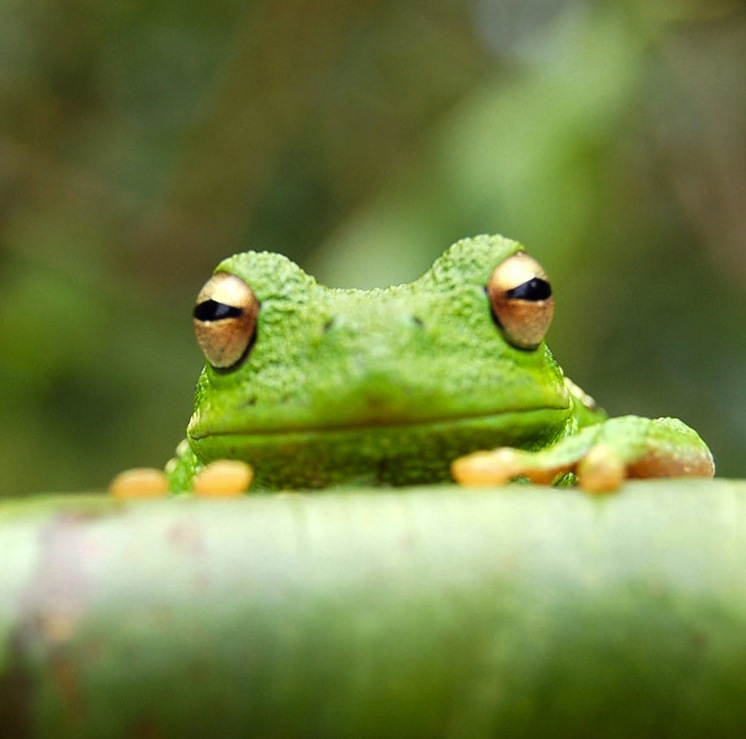
\includegraphics[width=0.3\textwidth]{frog.jpg}
\caption{\label{fig:frog}This frog was uploaded via the project menu.}
\end{figure}

\subsection{How to add Comments}

Comments can be added to your project by clicking on the comment icon in the toolbar above. % * <john.hammersley@gmail.com> 2016-07-03T09:54:16.211Z:
%
% Here's an example comment!
%
To reply to a comment, simply click the reply button in the lower right corner of the comment, and you can close them when you're done.

Comments can also be added to the margins of the compiled PDF using the todo command\todo{Here's a comment in the margin!}, as shown in the example on the right. You can also add inline comments:

\todo[inline, color=green!40]{This is an inline comment.}

\subsection{How to add Tables}

Use the table and tabular commands for basic tables --- see Table~\ref{tab:widgets}, for example. 

\begin{table}[h!]
\centering
\begin{tabular}{l|r}
Item & Quantity \\\hline
Widgets & 42 \\
Gadgets & 13
\end{tabular}
\caption{\label{tab:widgets}An example table.}
\end{table}



\bibliographystyle{apalike}
\bibliography{refsSpatial}

\end{document}